\documentclass{beamer}

\usepackage[utf8]{inputenc}
\usepackage[spanish]{babel}

\usepackage{graphicx}
\graphicspath{ {./img/} }

\usepackage{tkz-graph}
\usepackage{chessboard}

\title{Probabilidad y Cadenas de Markov}
\author{F. Galileo Cappella Lewi}
\date[PC2 2023]{Programación Competitiva 2\\\today}

\newcommand{\tab}{\phantom{mm}}
\newcommand{\chess}[1]{\chessboard[addpieces={R#1}]}
\newcommand{\tchess}[1]{\chessboard[tinyboard, addpieces={R#1}]}

% Configurando beamer
\usetheme{Boadilla}
\AtBeginSection[]{
  \begin{frame}
    \frametitle{Table of Contents}
    \tableofcontents[currentsection]
  \end{frame}
}

\usepackage{hyperref}
\hypersetup{
  colorlinks=true,
  linkcolor=blue,
  filecolor=magenta,      
  urlcolor=cyan,
}

\begin{document}

\frame{\titlepage}

\begin{frame}
  \frametitle{Table of Contents}
  \tableofcontents
\end{frame}

\newcommand{\SECTIONA}{Introducción a la probabilidad}
\section{\SECTIONA}

\begin{frame}
  \frametitle{\SECTIONA}

  La probabilidad es una forma de medir y pensar sobre la probabilidad de que pasen eventos. \pause Hay tres casos:
  \begin{itemize}
    \item<2-> Un evento imposible, con probabilidad 0
    \item<3-> Un evento que sí o sí sucede, con probabilidad 1
    \item<4-> Y un evento que capaz sucede, con probabilidad entre 0 y 1.
  \end{itemize} \pause \pause \pause % TODO: Sacar este hack, sino me aparece lo de abajo antes que el <4->
  La forma en la que definimos la probabilidad \(P\) de un \textbf{evento} \(E\) en un \textbf{espacio} \(S\) de posibilidades es la frecuencia con la que pasa. Es decir:
  \begin{gather*}
    0 \leq P(E) \leq 1 \\
    P(E) = \dfrac{|\{s \in S \text{ tal que ocurre } E \text{ en } s\}|}{|S|}
  \end{gather*}
\end{frame}

\begin{frame}
  \frametitle{\SECTIONA}
  \framesubtitle{Ejemplos de probabilidades}

  Por ejemplo, tirando un dado de seis caras el resultado es un entero entre 1 y 6, el espacio \(S = \{1, 2, 3, 4, 5, 6\}\). \pause Así tenemos que entonces al tirar un dado:
  \begin{itemize}
    \item<2-> \(P(\text{''sale un 4''}) = \dfrac{|\{4\}|}{|\{1, 2, 3, 4, 5, 6\}|} = \dfrac{1}{6}\). Similar para cualquiera de las seis caras.
    \item<3-> \(P(\text{''no sale un 6''}) = \dfrac{|\{1, 2, 3, 4, 5\}|}{|\{1, 2, 3, 4, 5, 6\}|} = \dfrac{5}{6}\). Similar para cualquiera de las seis caras.
    \item<4-> \(P(\text{''sale par''}) = \dfrac{|\{2, 4, 6\}|}{|\{1, 2, 3, 4, 5, 6\}|} = \dfrac{3}{6} = \dfrac{1}{2}\). Similar para que salga impar.
  \end{itemize}
\end{frame}

\subsection{Calculando probabilidades}

\begin{frame}
  \frametitle{\SECTIONA}
  \framesubtitle{Calculando probabilidades}

  Para calcular la probabilidad de un evento podemos o usar combinatoria o simular el proceso que genera al evento. \pause \\
  Como ejemplo vamos a calcular la probabilidad de sacar tres cartas del mismo valor de un mazo de 48 cartas bien mezclado.
\end{frame}

\begin{frame}
  \frametitle{\SECTIONA}
  \framesubtitle{Calculando probabilidades usando combinatoria}

  Este es el mismo método que vimos para los dados. \pause \\
  Hay \(\binom{48}{3}\) formas de agarrar tres cartas cualquieras del mazo. \pause \\
  Y como hay \(12\) posibles valores para las cartas y \(\binom{4}{3}\) formas de agarrar 3 palos de los cuatro palos posibles. Queda que hay \(12\binom{4}{3}\) casos en los que se cumple lo pedido. \pause \\
  Por lo que la probabilidad del evento es:
  \begin{gather*}
    \dfrac{12\binom{4}{3}}{\binom{48}{3}} = \dfrac{12 \cdot 4}{17296} = \dfrac{48}{17296} = \dfrac{3}{1081} \approx 0.0028 = 0.28\%
  \end{gather*}
\end{frame}

\begin{frame}
  \frametitle{\SECTIONA}
  \framesubtitle{Calculando probabilidades simulando el evento}

  En este método simulamos el proceso que genera al evento. \pause Que en este caso consiste de tres pasos en los que levantamos una carta en cada uno. Donde queremos que cada paso mantenga el evento deseado. \pause \\
  Agarrando la primera carta no importa cual salga, porque no hay ninguna restricción. \pause \\
  Agarrando la segunda de las 47 cartas restantes sólo nos sirven 3, por lo que hay \(\frac{3}{47}\) chances de que siga el evento. \pause \\
  Y agarrando la tercera carta, similarmente, quedan 46 cartas y sólo nos sirven 2, por lo que hay \(\frac{2}{46}\) chances. \pause \\ Por lo que la probabilidad del evento es:
  \begin{gather*}
    1 \cdot \dfrac{3}{47} \cdot \dfrac{2}{46} = \dfrac{3}{1081} \approx 0.0028 = 0.28\%
  \end{gather*}
\end{frame}

\subsection{Operaciones entre probabilidades}

\begin{frame}
  \frametitle{\SECTIONA}
  \framesubtitle{Operaciones entre probabilidades}

  Hay tres operaciones principales para las probabilidades:
  \begin{itemize}
    \item<2-> El \textbf{complemento} de un evento \(\bar{E}\), que son los casos en los que no pasa el evento \(E\): \(P(\bar{E}) = 1 - P(E)\).
    \item<3-> La \textbf{intersección} de dos eventos, que son los casos en los que pasan ambos a la vez: \(P(E_{1} \cap E_{2})\), la ecuación la vemos en un par de slides.
    \item<4-> Y la \textbf{unión} de dos eventos, que son los casos en los que pasa uno o el otro (o ambos): \(P(E_{1} \cup E_{2}) = P(E_{1}) + P(E_{2}) - P(E_{1} \cap E_{2})\). \pause \\
      Restamos los casos en los que pasan ambos, ya que los estaríamos contando dos veces al sumarlos.
  \end{itemize}
\end{frame}

\begin{frame}
  \frametitle{\SECTIONA}
  \framesubtitle{Probabilidad condicional}

  La \textbf{probabilidad condicional} de un evento \(A\) dado otro evento \(B\) es:
  \begin{gather*}
    P(A | B) = \dfrac{P(A \cap B)}{P(B)}
  \end{gather*}
  Esta es la probabilidad de que pasen \(A\) y \(B\) dado que pasa \(B\). \pause \\
  Con esto se puede derivar la probabilidad de la intersección de dos eventos como:
  \begin{gather*}
    P(A \cap B) = P(A | B) \cdot P(B)
  \end{gather*} \pause
  Y cuando sucede que \(P(A|B) = P(A)\) y \(P(B|A) = P(B)\) se los define como eventos \textbf{independientes} entre sí, y se tiene que:
  \begin{gather*}
    P(A \cap B) = P(A) \cdot P(B)
  \end{gather*}
\end{frame}

\subsection{Variables aleatorias}

\begin{frame}
  \frametitle{\SECTIONA}
  \framesubtitle{Variables aleatorias}

  Una \textbf{variable aleatoria (VA)} es un valor generado por un proceso aleatorio. Por ejemplo, si tiramos dos dados, la suma de sus valores es una VA. \\
  Para una VA \(X\) y un valor \(x\) de ella, podemos definir \(P(X = x)\) como la probabilidad del evento en el que \(X\) vale \(x\). \pause \\

  Sobre la VA \(X\), definimos la \textbf{esperanza} \(E(X)\) como el valor que tiene en promedio. Y se calcula:
  \begin{gather*}
    E(X) = \sum_{x}x \cdot P(X = x)
  \end{gather*}
  para \(x\) recorriendo todos los valores posibles de \(X\). \pause \\
  Por ejemplo, al tirar un dado:
  \begin{gather*}
    E(X) = 1 \cdot \dfrac{1}{6} + 2 \cdot \dfrac{1}{6} + 3 \cdot \dfrac{1}{6} + 4 \cdot \dfrac{1}{6} + 5 \cdot \dfrac{1}{6} + 6 \cdot \dfrac{1}{6} = \dfrac{7}{2}
  \end{gather*}
\end{frame}

\begin{frame}
  \frametitle{\SECTIONA}
  \framesubtitle{Linealidad de la esperanza}

  Una propiedad útil de la esperanza es su \textbf{linealidad}. Es decir:
  \begin{gather*}
    E(X_{1} + X_{2} + \ldots + X_{k}) = E(X_{1}) + E(X_{2}) + \ldots + E(X_{k})
  \end{gather*} \pause

  Por ejemplo al tirar dos dados, si definimos a \(X_{1}\) como el valor del primer dado, y \(X_{2}\) como el del segundo, podemos calcular la esperanza de la suma usando la linealidad:
  \begin{gather*}
    E(X_{1} + X_{2}) = E(X_{1}) + E(X_{2}) = \dfrac{7}{2} + \frac{7}{2} = 7
  \end{gather*} \pause

  No hace falta que las VA sean independientes. Esto vale SIEMPRE.
\end{frame}

\subsection{Distribuciones}

\begin{frame}
  \frametitle{\SECTIONA}
  \framesubtitle{Distribuciones}

  Una \textbf{distribución} es una forma de describir una VA. Nos permite saber para cada \(x\) cuánto vale \(P(X = x)\). Las distribuciones se pueden dar con una tabla, que para cada valor muestre la probabilidad, o con una fórmula que permite calcularla en cada valor de \(x\). \pause \\
  Hay varias distribuciones ya conocidas, nos son relevantes cuatro.
\end{frame}

\begin{frame}
  \frametitle{\SECTIONA}
  \framesubtitle{Distribuciones: Bernoulli y Binomial}

  \begin{itemize}
    \item VA de \textbf{Bernoulli}: Vale 0 ó 1, con probabilidad \(p\) de valer 1. \\
      Ej: Tirar una moneda y considerar cara como 0 y ceca como 1.
      \begin{gather*}
        P(X = 1) = p \\
        P(X = 0) = 1 - p \\
        E(X) = p
      \end{gather*}
    \item<2-> VA \textbf{binomial}: Es la suma de \(n\) Bernoullis. \\
      Ej: Tirar una moneda \(n\) veces y sumar sus resultados.
      \begin{gather*}
        P(X = x) = \binom{n}{x} \cdot p^{x} \cdot (1 - p)^{n - x} \\
        E(X) = np
      \end{gather*}
  \end{itemize}
\end{frame}

\begin{frame}
  \frametitle{\SECTIONA}
  \framesubtitle{Distribuciones: Geométrica y Uniforme}

  \begin{itemize}
    \item VA \textbf{geométrica}: En un proceso que evalúa Bernoullis de probabilidad \(p\), representa la cantidad de intentos hasta el primer éxito. \\
      Ej: Tirar una moneda hasta que salga un 1 (ceca).
      \begin{gather*}
        P(X = x) = (1 - p)^{x - 1} \cdot p \\
        E(X) = \dfrac{1}{p}
      \end{gather*}
    \item<2-> VA \textbf{uniforme}: Esta la usamos seguido en programación. La VA puede valer un entero cualquiera en el rango \([a, b]\) con misma probabilidad. \\
      Ej: Tirar una moneda \(n\) veces y sumar sus resultados.
      \begin{gather*}
        P(X = x) = \begin{cases} \dfrac{1}{b - a} & \text{if } a \leq x \leq b \\ 0 & \text{otherwise} \\ \end{cases} \\
        E(X) = \dfrac{a + b}{2}
      \end{gather*}
  \end{itemize}
\end{frame}

\newcommand{\SECTIONB}{Problemas de Probabilidad}
\section{\SECTIONB}
\newcommand{\EJA}{\href{https://cses.fi/problemset/task/1725/}{CSES 1725 - Dice Probability}}

\subsection{CSES 1725 - Dice Probability}

\begin{frame}
  \frametitle{\SECTIONB}
  \framesubtitle{\EJA}

  Tirando un dado de seis caras \(n\) veces. ¿Cual es la probabilidad de que la suma de los resultados esté entre \(a\) y \(b\)? \pause \\
  Primero nombramos a la VA \(S_{n}\) como la suma de las \(n\) tiradas. Entonces queremos calcular \(P(a \leq S_{n} \leq b)\). \pause \\
  Esto es lo mismo que \(P(S_{n} = a) + P(S_{n} = a+1) + \ldots + P(S_{n} = b)\). \pause \\
  Ahora \(n = 1\) es fácil, ya que \(S_{1}\) es lo mismo que el resultado de tirar un sólo dado. \\
  ¿Cómo hacemos para \(n > 1\)?

\end{frame}

\begin{frame}
  \frametitle{\SECTIONB}
  \framesubtitle{\EJA para \(n > 1\)}

  Tomamos \(X_{j}\) al resultado de la \(j\)-ésima tirada. \\
  Al tirar el \(j\)-ésimo dado ya tenemos la suma parcial \(S_{j} = X_{1} + X_{2} + \ldots + X_{j}\). \pause \\
  Esto nos permite calcular la probabilidad de los valores de la \((j+1)\)-ésima tirada como:
  {\small
  \begin{align*}
    P(S_{j+1} = x) &= P(X_{j+1} = 1 | S_{j} = x - 1) + P(X_{j+1} = 2 | S_{j} = x - 2) + \ldots \\
                  & + P(X_{j+1} = 6 | S_{j} = x - 6)  \\
                  &= \sum_{i = 1}^{6}P(X_{j+1} = i | S_{j} = x - i) \\
                  &= \sum_{i = 1}^{6}P(X_{j+1} = i) \cdot P(S_{j} = x - i) \\
                  &= \sum_{i = 1}^{6}\frac{1}{6} \cdot P(S_{j} = x - i) = \frac{1}{6}\sum_{i = 1}^{6}P(S_{j} = x - i) \\
  \end{align*}
  }%
\end{frame}

\begin{frame}
  \frametitle{\SECTIONB}
  \framesubtitle{\EJA para \(n > 1\)}

  Quedándonos con:
  \begin{gather*}
    P(S_{j+1} = x) = \frac{1}{6}\sum_{i = 1}^{6}P(S_{j} = x - i)
  \end{gather*}
  Y resaltando que \(j \leq S_{j} \leq 6j\). \\
  Podemos entonces calcular \(P(S_{n} = x)\) recursivamente llamando a la siguiente función con \(f(n, x)\):
  \begin{gather*}
    f(j, x) = \begin{cases}
      0 & \text{if } \neg(j \leq x \leq 6j) \\
      \frac{1}{6} & \text{if } j = 1 \\
      \frac{1}{6}\sum_{i = 1}^{6}f(j-1, x-i) & \text{otherwise} \\
    \end{cases}
  \end{gather*} \pause
  Ver código.
\end{frame}

\newcommand{\EJB}{\href{https://codeforces.com/group/YjFmW2O15Q/contest/101919}{TAP 2018 E, Estacionamiento}}

\begin{frame}
  \frametitle{\SECTIONB}
  \framesubtitle{\EJB}

  Tenemos \(M\) cuadras a nuestra izquierda y a nuestra derecha y queremos encontrar nuestro auto. Para cada cuadra sabemos la probabilidad de que el auto se encuentre en ella. Asumiendo que nos movemos de forma óptima, queremos calcular la cantidad mínima de cuadras que caminaríamos en promedio hasta encontrarlo.

\end{frame}

\begin{frame}
  \frametitle{\SECTIONB}
  \framesubtitle{\EJB}

  En cada posición queremos decidir si movernos hacia la izquierda o hacia la derecha. \pause Y obviamente queremos tomar la dirección que nos de la cantidad mínima esperada de cuadras que caminaríamos. \pause \\
  Esto es el mismo problema que tenemos ahora mismo pero con un poco más de información (la de ya haber caminado por donde nos movamos). Por lo que es claro que se resuelve con recursión.
\end{frame}

\begin{frame}
  \frametitle{\SECTIONB}
  \framesubtitle{\EJB}

  En específico vamos a tener que llamar \(f(M, M, \text{L})\). Con \(p(l, r) = P(\text{No esté en } [l, r]) = 1 - P(\text{Sí esté en } [l, r])\) y:
  \begin{gather*}
    f(l, r, dir) = \begin{cases}
      \infty & \text{if } l < 0 \lor r \geq 2M \\
      0 & \text{if } l == 0 \land r == 2M-1 \\
      min( \\
      \tab mantenerDir(l, r, dir), \\
      \tab cambiarDir(l, r, dir) \\
      ) & \text{otherwise}
    \end{cases}
  \end{gather*}

  \begin{gather*}
    mantenerDir(l, r, dir) = \begin{cases}
      p(l, r) + f(l-1, r, \text{L}) & \text{if } dir = \text{L} \\
      p(l, r) + f(l, r+1, \text{R}) & \text{if } dir = \text{R}
    \end{cases}
  \end{gather*}

  \begin{gather*}
    cambiarDir(l, r, dir) = \begin{cases}
      p(l, r) \cdot |[l, r]| + f(l-1, r, \text{R}) & \text{if } dir = \text{L} \\
      p(l, r) \cdot |[l, r]| + f(l, r+1, \text{L}) & \text{if } dir = \text{R}
    \end{cases}
  \end{gather*}
\end{frame}

\newcommand{\SECTIONC}{Cadenas de Markov}
\section{\SECTIONC}

\begin{frame}
  \frametitle{\SECTIONC}
  \framesubtitle{Una apuesta}

  Supongamos que tienen \$100 y les ofrezco una apuesta donde vamos a tirar una moneda 100 veces seguidas. Cada vez que salga cara su riqueza sube un 50\%, y cada vez que salga cruz su riqueza decrementa un 40\%. ¿La tomarían?
\end{frame}

\begin{frame}
  \frametitle{\SECTIONC}
  \framesubtitle{Una apuesta... Buena}

  En un principio podemos calcular la ganancia esperada: Para la primera tirada tenemos un 50\% chances de ganar \$50, y un 50\% chances de perder \$40. Por lo que esperaríamos ganar:
  \begin{gather*}
    \$50 \cdot 50\% + \$(-40) \cdot 50\% = \$5 = \$100 \cdot \%5
  \end{gather*}
  \pause El valor de la apuesta va a cambiar en las tiradas futuras, pero en todas vamos a tener una ganancia esperada del 5\%. Por lo que en promedio esperaríamos ganar un 5\% por tirada.
\end{frame}

\begin{frame}
  \frametitle{\SECTIONC}
  \framesubtitle{Una apuesta... Buena}

  Simulando esta apuesta para 10000 personas podemos ver que este promedio se cumple.

  \begin{figure}[H]
    \centering
    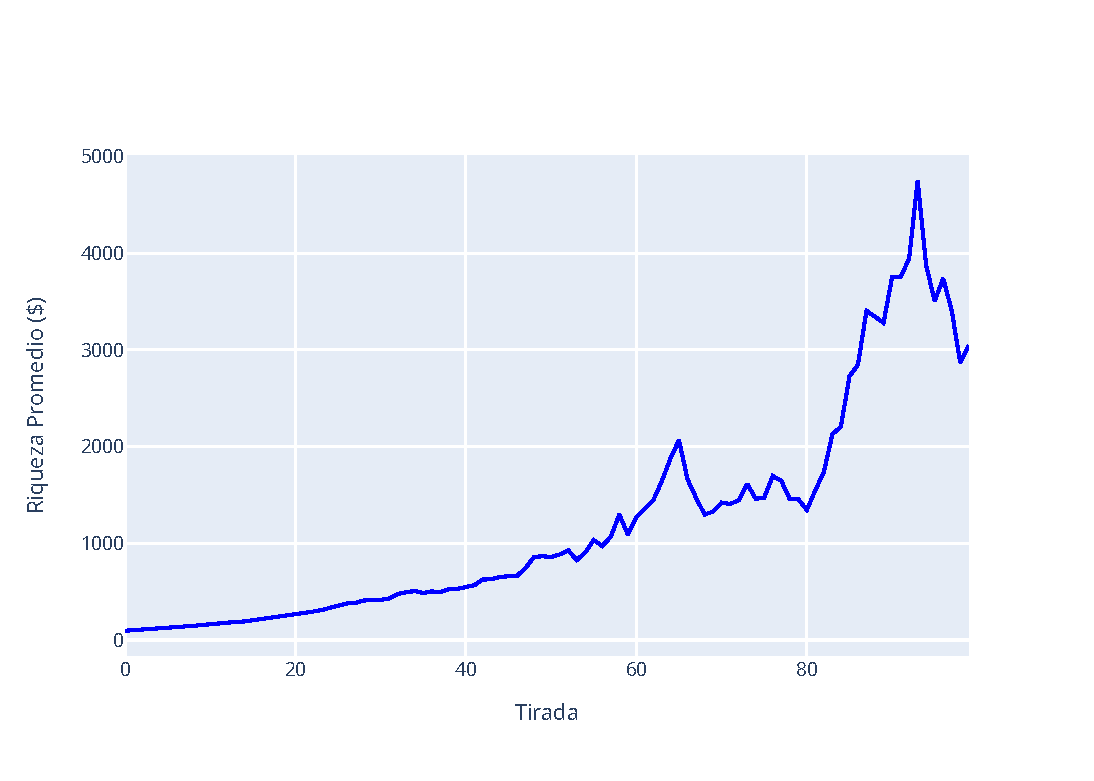
\includegraphics[scale=0.5]{img/mean.pdf}
  \end{figure}
\end{frame}

\begin{frame}
  \frametitle{\SECTIONC}
  \framesubtitle{Una apuesta... Buena?}

  Pero mirándolo desde otra perspectiva, si revisamos la trayectoria de 20 de estas personas, notamos que aunque a un par les va bien la mayoría no alcanza tanta riqueza.

  \begin{figure}[H]
    \centering
    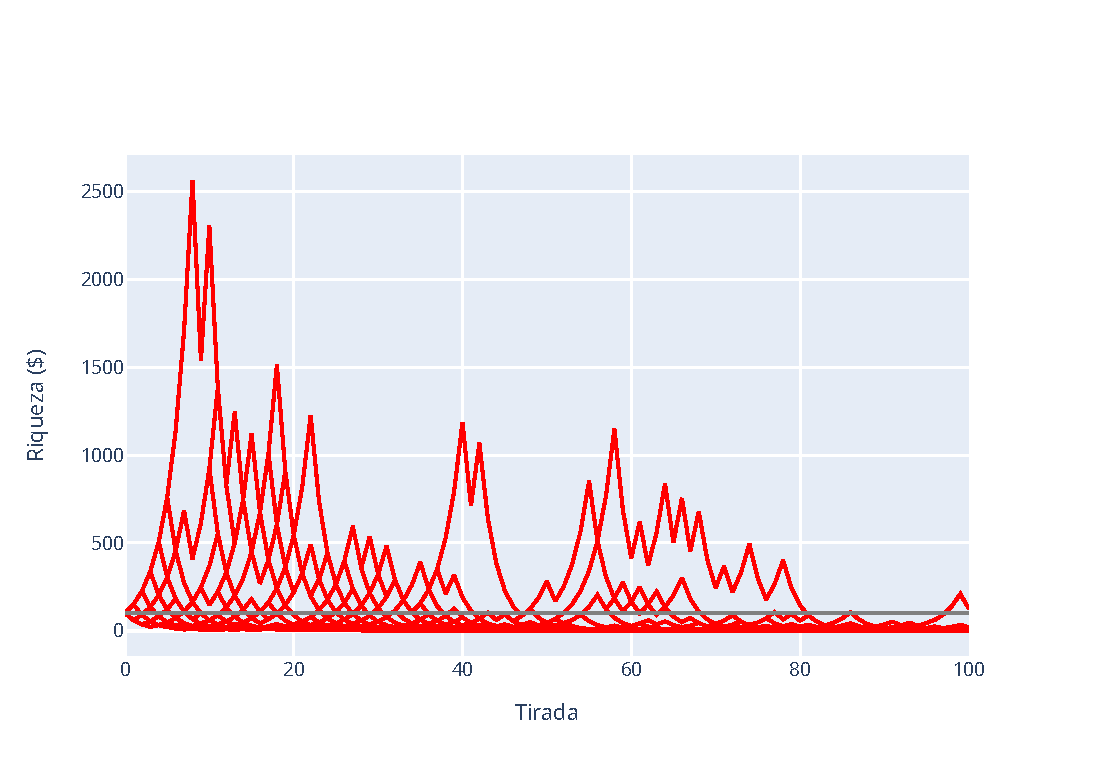
\includegraphics[scale=0.5]{img/paths.pdf}
  \end{figure}
\end{frame}

\begin{frame}
  \frametitle{\SECTIONC}
  \framesubtitle{Una apuesta... Mala}

  De hecho, si lo miramos en escala logarítmica, se resalta que la mediana perdió casi todo su riqueza.

  \begin{figure}[H]
    \centering
    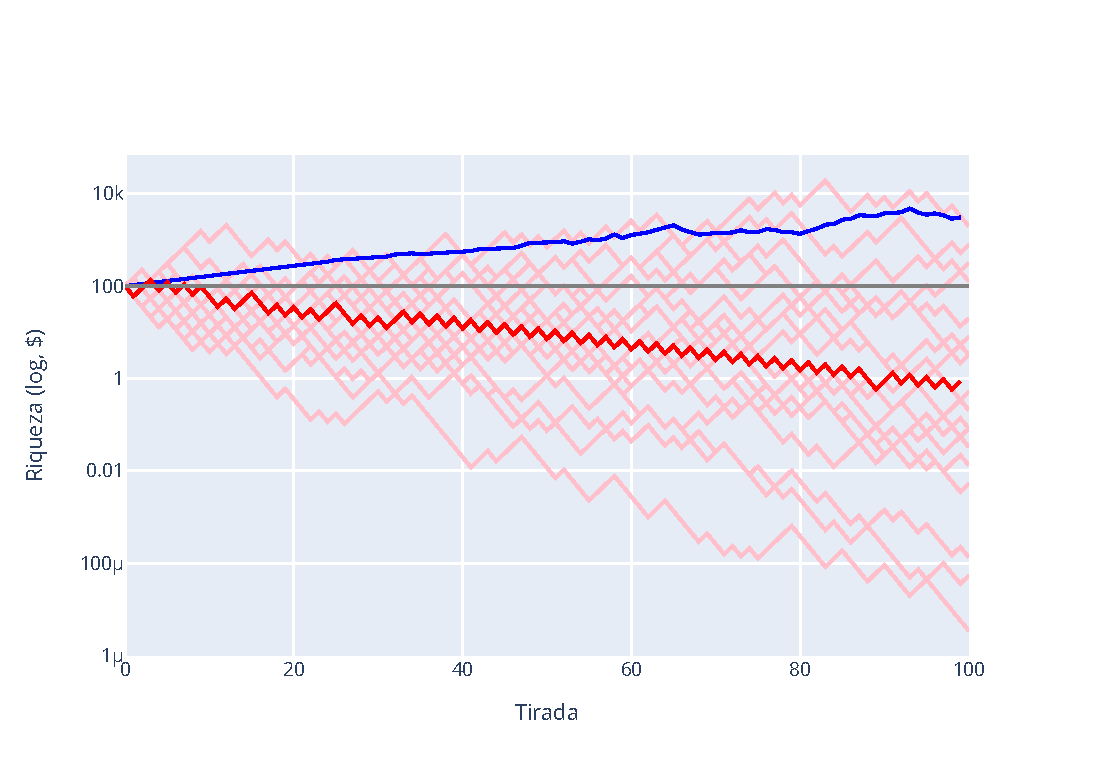
\includegraphics[scale=0.5]{img/logPaths.pdf}
  \end{figure}
\end{frame}

\begin{frame}
  \frametitle{\SECTIONC}
  \framesubtitle{Gambler's Ruin y ergodicidad}

  A este problema se lo conoce como la Gambler's Ruin (Ruina del Apostador). Y es un ejemplo de un sistema no-ergódico. \pause \\
  Un sistema ergódico es un sistema donde el promedio individual sobre el tiempo converge al promedio grupal. \pause La mayoría de los sistemas reales son no-ergódicos. \pause \\
  Ver un problema así nos resalta que la probabilidad no es tan directa como la solemos pensar. No es suficiente con quedarse con el cálculo de la ganancia promedio.
\end{frame}

\setchessboard{maxfield=c3, showmover=false, vlabel=false, hlabel=false}

\begin{frame}
  \frametitle{\SECTIONC}
  \framesubtitle{Ahora sí: Markov}

  Problemas como el anterior se pueden representar como lo que se conoce como un modelo de Markov. Donde tenemos un estado que cambia aleatoriamente en base al estado anterior. \pause \\
  El caso anterior es complicado de representar, por lo que vamos a ver a otro sistema más fácil de representar.

\end{frame}

\newcommand{\GVertex}[4]{\Vertex[L=#1,x=#2,y=#3]{#4}}
\newcommand{\CVertex}[4]{\GVertex{\tchess{#1}}{#2}{#3}{#4}}
\newcommand{\TVertex}[5]{\GVertex{{$\langle #1, #2 \rangle$}}{#3}{#4}{#5}}

\newcommand{\GEdge}[3]{\Edge[label=#1](#2)(#3)}
\newcommand{\GBEdge}[3]{\Edge[style={bend left=30},label=#1](#2)(#3)}
\tikzset{EdgeStyle/.style = {->}}

\newcommand{\EJC}{Un robot a través del espejo}

\begin{frame}
  \frametitle{\SECTIONC}
  \framesubtitle{\EJC}

  Vamos a modelar a un robot que se mueve sobre un tablero como de ajedrez. \pause En específico va a empezar en la posición \(\langle 1, 1 \rangle\) en un tablero de \(3 \times 3\). En cada paso elije al azar a dónde se mueve entre los casilleros que tenga al lado. Se busca saber la probabilidad de que esté en algún casillero específico después de \(k\) pasos.

  \begin{figure}[H]
    \centering
    \chess{a1}
  \end{figure}
\end{frame}

\begin{frame}
  \frametitle{\SECTIONC}
  \framesubtitle{\EJC: Paso cero}

  \begin{figure}[H]
    \centering
    \scalebox{0.8}{
      \begin{tikzpicture}
        \CVertex{a1}{0}{0}{0}
      \end{tikzpicture}
    }
  \end{figure}
\end{frame}

\begin{frame}
  \frametitle{\SECTIONC}
  \framesubtitle{\EJC: Paso uno}

  \begin{figure}[H]
    \centering
    \scalebox{0.8}{
      \begin{tikzpicture}
        \CVertex{a1}{0}{0}{0}
          \CVertex{a2}{-3}{-3}{1}
          \CVertex{b1}{3}{-3}{2}

        \GEdge{$\frac{1}{2}$}{0}{1}
        \GEdge{$\frac{1}{2}$}{0}{2}
      \end{tikzpicture}
    }
  \end{figure}
\end{frame}

\begin{frame}
  \frametitle{\SECTIONC}
  \framesubtitle{\EJC: Paso dos}

  \begin{figure}[H]
    \centering
    \scalebox{0.8}{
      \begin{tikzpicture}
        \CVertex{a1}{0}{0}{0}
          \CVertex{a2}{-3}{-3}{1}
            \CVertex{a3}{-6}{-6}{3}
            \CVertex{b2}{0}{-6}{4}
          \CVertex{b1}{3}{-3}{2}
            \CVertex{c1}{6}{-6}{5}

        \GEdge{$\frac{1}{3}$}{1}{0}
        \GEdge{$\frac{1}{3}$}{1}{3}
        \GEdge{$\frac{1}{3}$}{1}{4}

        \GEdge{$\frac{1}{3}$}{2}{0}
        \GEdge{$\frac{1}{3}$}{2}{4}
        \GEdge{$\frac{1}{3}$}{2}{5}
      \end{tikzpicture}
    }
  \end{figure}
\end{frame}

\begin{frame}
  \frametitle{\SECTIONC}
  \framesubtitle{\EJC: Paso cero}

  \begin{figure}[H]
    \centering
    \begin{tikzpicture}
      \GVertex{1}{0}{0}{0}
      \GVertex{0}{2}{0}{1}
      \GVertex{0}{4}{0}{2}

      \GVertex{0}{0}{2}{3}
      \GVertex{0}{2}{2}{4}
      \GVertex{0}{4}{2}{5}

      \GVertex{0}{0}{4}{6}
      \GVertex{0}{2}{4}{7}
      \GVertex{0}{4}{4}{8}
    \end{tikzpicture}
  \end{figure}
\end{frame}

\begin{frame}
  \frametitle{\SECTIONC}
  \framesubtitle{\EJC: Paso uno}

  \begin{figure}[H]
    \centering
    \begin{tikzpicture}
      \GVertex{0}{0}{0}{0}
      \GVertex{$\frac{1}{2}$}{2}{0}{1}
      \GVertex{0}{4}{0}{2}

      \GVertex{$\frac{1}{2}$}{0}{2}{3}
      \GVertex{0}{2}{2}{4}
      \GVertex{0}{4}{2}{5}

      \GVertex{0}{0}{4}{6}
      \GVertex{0}{2}{4}{7}
      \GVertex{0}{4}{4}{8}

      \GEdge{$\frac{1}{2}$}{0}{1}
      \GEdge{$\frac{1}{2}$}{0}{3}
    \end{tikzpicture}
  \end{figure}
\end{frame}

\begin{frame}
  \frametitle{\SECTIONC}
  \framesubtitle{\EJC: Paso dos}

  \begin{figure}[H]
    \centering
    \begin{tikzpicture}
      \GVertex{$\frac{1}{3}$}{0}{0}{0}
      \GVertex{0}{2}{0}{1}
      \GVertex{$\frac{1}{6}$}{4}{0}{2}

      \GVertex{0}{0}{2}{3}
      \GVertex{$\frac{1}{3}$}{2}{2}{4}
      \GVertex{0}{4}{2}{5}

      \GVertex{$\frac{1}{6}$}{0}{4}{6}
      \GVertex{0}{2}{4}{7}
      \GVertex{0}{4}{4}{8}

      \GEdge{$\frac{1}{3}$}{1}{0}
      \GEdge{$\frac{1}{3}$}{1}{2}
      \GEdge{$\frac{1}{3}$}{1}{4}

      \GEdge{$\frac{1}{3}$}{3}{0}
      \GEdge{$\frac{1}{3}$}{3}{4}
      \GEdge{$\frac{1}{3}$}{3}{6}
    \end{tikzpicture}
  \end{figure}
\end{frame}

\begin{frame}
  \frametitle{\SECTIONC}
  \framesubtitle{\EJC: Full}

  \begin{figure}[H]
    \centering
    \begin{tikzpicture}
      \TVertex{1}{1}{0}{0}{0}
      \TVertex{2}{1}{2}{0}{1}
      \TVertex{3}{1}{4}{0}{2}

      \TVertex{1}{2}{0}{2}{3}
      \TVertex{2}{2}{2}{2}{4}
      \TVertex{3}{2}{4}{2}{5}

      \TVertex{1}{3}{0}{4}{6}
      \TVertex{2}{3}{2}{4}{7}
      \TVertex{3}{3}{4}{4}{8}

      \GBEdge{$\frac{1}{2}$}{0}{1}
      \GBEdge{$\frac{1}{2}$}{0}{3}

      \GBEdge{$\frac{1}{3}$}{1}{0}
      \GBEdge{$\frac{1}{3}$}{1}{2}
      \GBEdge{$\frac{1}{3}$}{1}{4}

      \GBEdge{$\frac{1}{2}$}{2}{1}
      \GBEdge{$\frac{1}{2}$}{2}{5}

      \GBEdge{$\frac{1}{3}$}{3}{0}
      \GBEdge{$\frac{1}{3}$}{3}{4}
      \GBEdge{$\frac{1}{3}$}{3}{6}

      \GBEdge{$\frac{1}{4}$}{4}{1}
      \GBEdge{$\frac{1}{4}$}{4}{3}
      \GBEdge{$\frac{1}{4}$}{4}{5}
      \GBEdge{$\frac{1}{4}$}{4}{7}

      \GBEdge{$\frac{1}{3}$}{5}{2}
      \GBEdge{$\frac{1}{3}$}{5}{4}
      \GBEdge{$\frac{1}{3}$}{5}{8}

      \GBEdge{$\frac{1}{2}$}{6}{3}
      \GBEdge{$\frac{1}{2}$}{6}{7}

      \GBEdge{$\frac{1}{3}$}{7}{4}
      \GBEdge{$\frac{1}{3}$}{7}{6}
      \GBEdge{$\frac{1}{3}$}{7}{8}

      \GBEdge{$\frac{1}{2}$}{8}{5}
      \GBEdge{$\frac{1}{2}$}{8}{7}
    \end{tikzpicture}
  \end{figure}
\end{frame}

\begin{frame}
  \frametitle{\SECTIONC}
  \framesubtitle{\EJC: Matriz}

  \begin{gather*}
    \overbrace{\begin{pmatrix}
        0 & \frac{1}{3} & 0 & \frac{1}{3} & 0 & 0 & 0 & 0 & 0  \\
        \frac{1}{2} & 0 & \frac{1}{2} & 0 & \frac{1}{4} & 0 & 0 & 0 & 0  \\
        0 & \frac{1}{3} & 0 & 0 & 0 & \frac{1}{3} & 0 & 0 & 0  \\
        \frac{1}{2} & 0 & 0 & 0 & \frac{1}{4} & 0 & \frac{1}{2} & 0 & 0  \\
        0 & \frac{1}{3} & 0 & \frac{1}{3} & 0 & \frac{1}{3} & 0 & \frac{1}{3} & 0  \\
        0 & 0 & \frac{1}{2} & 0 & \frac{1}{4} & 0 & 0 & 0 & \frac{1}{2} \\
        0 & 0 & 0 & \frac{1}{3} & 0 & 0 & 0 & \frac{1}{3} & 0  \\
        0 & 0 & 0 & 0 & \frac{1}{4} & 0 & \frac{1}{2} & 0 & \frac{1}{2} \\
        0 & 0 & 0 & 0 & 0 & \frac{1}{3} & 0 & \frac{1}{3} & 0
    \end{pmatrix}}^{\text{Matriz de transición}}
    \overbrace{\begin{pmatrix}
      0 \\ 0 \\ 0 \\ 0 \\ 0 \\ 0 \\ 0 \\ 0 \\ 1 
    \end{pmatrix}}^{\text{Este estado (\(\langle 1, 1 \rangle\))}}
  \end{gather*}
\end{frame}

\begin{frame}
  \frametitle{\SECTIONC}
  \framesubtitle{\EJC: Matriz}

  \begin{gather*}
    \overbrace{\begin{pmatrix}
        0 & \frac{1}{3} & 0 & \frac{1}{3} & 0 & 0 & 0 & 0 & 0  \\
        \frac{1}{2} & 0 & \frac{1}{2} & 0 & \frac{1}{4} & 0 & 0 & 0 & 0  \\
        0 & \frac{1}{3} & 0 & 0 & 0 & \frac{1}{3} & 0 & 0 & 0  \\
        \frac{1}{2} & 0 & 0 & 0 & \frac{1}{4} & 0 & \frac{1}{2} & 0 & 0  \\
        0 & \frac{1}{3} & 0 & \frac{1}{3} & 0 & \frac{1}{3} & 0 & \frac{1}{3} & 0  \\
        0 & 0 & \frac{1}{2} & 0 & \frac{1}{4} & 0 & 0 & 0 & \frac{1}{2} \\
        0 & 0 & 0 & \frac{1}{3} & 0 & 0 & 0 & \frac{1}{3} & 0  \\
        0 & 0 & 0 & 0 & \frac{1}{4} & 0 & \frac{1}{2} & 0 & \frac{1}{2} \\
        0 & 0 & 0 & 0 & 0 & \frac{1}{3} & 0 & \frac{1}{3} & 0
    \end{pmatrix}}^{\text{Matriz de transición}}
    \overbrace{\begin{pmatrix}
      0 \\ 0 \\ 0 \\ 0 \\ 0 \\ 0 \\ 0 \\ 0 \\ 1 
    \end{pmatrix}}^{\text{Este estado (\(\langle 1, 1 \rangle\))}}
    =
    \overbrace{\begin{pmatrix}
      0 \\ 0 \\ 0 \\ 0 \\ 0 \\ \frac{1}{2} \\ 0 \\ \frac{1}{2} \\ 0 
    \end{pmatrix}}^{\text{Siguiente estado}}
  \end{gather*}
\end{frame}

\begin{frame}
  \frametitle{\SECTIONC}
  \framesubtitle{\EJC: Resultado}

  \begin{gather*}
    M^{k} v_{0} = \overbrace{v_{k}}^{\text{Distribución del \(k\)-ésimo estado}}
  \end{gather*} \pause
  Por lo que el resultado a lo pedido es
  \begin{gather*}
    P(\text{Esté en la posición } \langle r, c \rangle \text{ en el \(k\)-ésimo } k \text{ paso}) = (M^{k}v_{0})_{3r + c} = (v_{k})_{3r + c}
  \end{gather*}
\end{frame}

%TODO: Alguna conclusión o generalización?

\newcommand{\SECTIOND}{Problemas de Markov}
\section{\SECTIOND}
\newcommand{\EJD}{\href{https://cses.fi/problemset/view/1726/}{CSES 1726 - Moving Robots}}

\begin{frame}
  \frametitle{\SECTIOND}
  \framesubtitle{\EJD}

  En cada casillero de un tablero de ajedrez de \(8 \times 8\) se tiene un robot. En cada paso todos los robots se mueven aleatoriamente a uno de sus casilleros adyacentes. Se pueden tener varios robots en un mismo casillero. \\
  Se busca calcular la cantidad esperada de casilleros vacíos después de \(k\) pasos. \pause \\
  Este problema se parece mucho al que hicimos antes, sólo que ahora en lugar de tener un sólo robot tenemos varios, y el tablero es más grande.
\end{frame}

\begin{frame}
  \frametitle{\SECTIOND}
  \framesubtitle{\EJD, para cada casillero}

  Primero vamos a querer simular a cada robot, para calcular su distribución después de \(k\) pasos. \pause Esto es simple: Calculamos la matriz de transición, la elevamos a \(k\), y luego la multiplicamos por cada vector inicial. \pause \\
  Una vez que tenemos las distribuciones para cada robot, podemos calcular la probabilidad de que no haya ningún robot en un casillero como el producto de el inverso de las probabilidades de todos los robots. \pause
  \begin{align*}
    P(\text{No haya ningún en } \langle r, c \rangle) &= \bigcap_{0 \leq i < 64} P(\text{El robot } i \text{ no esté en } \langle r, c \rangle) \\
                                                      &= \prod_{0 \leq i < 64}P(\text{El robot } i \text{ no esté en } \langle r, c \rangle) \\
                                                      &= \prod_{0 \leq i < 64}(1 - P(\text{El robot } i \text{ esté en } \langle r, c \rangle)) \\
                                                      &= \prod_{0 \leq i < 64}(1 - (M^{k}v_{i,0})_{8r + c}) \\
  \end{align*}
\end{frame}

\begin{frame}
  \frametitle{\SECTIONC}
  \framesubtitle{\EJD, solución}

  Y ahora, teniendo la probabilidad de que no haya ningún robot en cada casillero. Tenemos que la cantidad esperada de casilleros vacíos es la suma de estas probabilidades. \pause 
  \begin{gather*}
    E(\text{Vacíos después de \(k\) pasos}) = \sum_{\langle r, c \rangle}1 \cdot P(\text{No haya ningún en } \langle r, c \rangle)
  \end{gather*}
\end{frame}

\section{Notas finales}

\begin{frame}
  \frametitle{Bibliografía y referencias}
  
  \begin{itemize}
  \item \textbf{Training Camp 2023}, clase por Caro Lang \\
  \item \textbf{Competitive Programmer's Handbook}, Antti Laaksonen de CSES \\
      \href{https://cses.fi/book/book.pdf}{https://cses.fi/book/book.pdf}
  \item \textbf{The Probability Distribution of the Sum of Several Dice: Slot Applications}, Ashok K. Singh, Rohan J. Dalpatadu, Anthony F. Lucas \\
      \href{https://digitalscholarship.unlv.edu/cgi/viewcontent.cgi?article=1025&context=grrj}{https://digitalscholarship.unlv.edu/cgi/viewcontent.cgi?article=1025\&context=grrj}
    \item \textbf{Ergodicity economics: a primer}, Jason Collins \\
      \href{https://www.jasoncollins.blog/posts/ergodicity-economics-a-primer}{https://www.jasoncollins.blog/posts/ergodicity-economics-a-primer}
  \end{itemize}
\end{frame}

\end{document}
